\subsection{Hintergrund der Arbeit}
\subsubsection{Photogrammetrische Aufzeichnungen des SABA Geländes}
Das studentische Forschungsprojekt aus dem Wintersemester 19/20 \cite{reich2020} befasst sich mit  der Photogrammetrischen Aufzeichnung des SABA-Geländes in Villingen-Schwenningen. SABA (Schwarzwälder Apparate-Bau-Anstalt) war ein deutsches Unternehmen, das unter anderem elektronische Geräte für den Rundfunk herstellte. Der Entwicklungs- und Produktionsstandort war das Gebäude in Villingen. Aufgrund der Größe des Unternehmens (mehr als 6000 Mitarbeiter), hatte SABA eine große Bedeutung für die Stadt. 1986 wurde das Unternehmen aufgelöst, bis das Gebäude am 11. August 2021 abgerissen wurde.\footnote{https://dewiki.de/Lexikon/SABA, zuletzt aufgerufen am 17.03.2022} 

Mithilfe von Drohnen- und Bodenaufnahmen wird ein 3D Modell des SABA Geländes mit photgrammetrischen Algorithmen erzeugt. \textit{Regard3D} \footnote{https://www.regard3d.org/}, \textit{RealityCapture} \footnote{https://www.capturingreality.com/}, \textit{VisualSFM} \footnote{http://ccwu.me/vsfm/} und \textit{Meshroom} \footnote{https://github.com/alicevision/meshroom} werden im Projektverlauf genutzt und verglichen, wobei \textit{Meshroom} als kostenlose Open-Source Software hauptsächlich genutzt wird. Das Hauptgebäude wird nach der Erstellung des Meshes aus \textit{Meshroom} neu modelliert. Aufgrund der hohen Dichte der Vertices ist die Aufteilung der einzelnen Gebäude-Elemente wie Fenster, Wand und Türen schwierig. Durch eine Neumodellierung wird das Modell klarer und die Texturierung wird vereinfacht. Als Grundlage dient dabei das generierte Mesh aus \textit{Meshroom}. Als Modellierunssoftware wird \textit{Blender} benutzt.\footnote{https://www.blender.org/} In Abbildung \ref{fig:SABA3DModell} ist das fertige 3D Modell zu sehen.

\begin{figure}[ht]
    \centering
    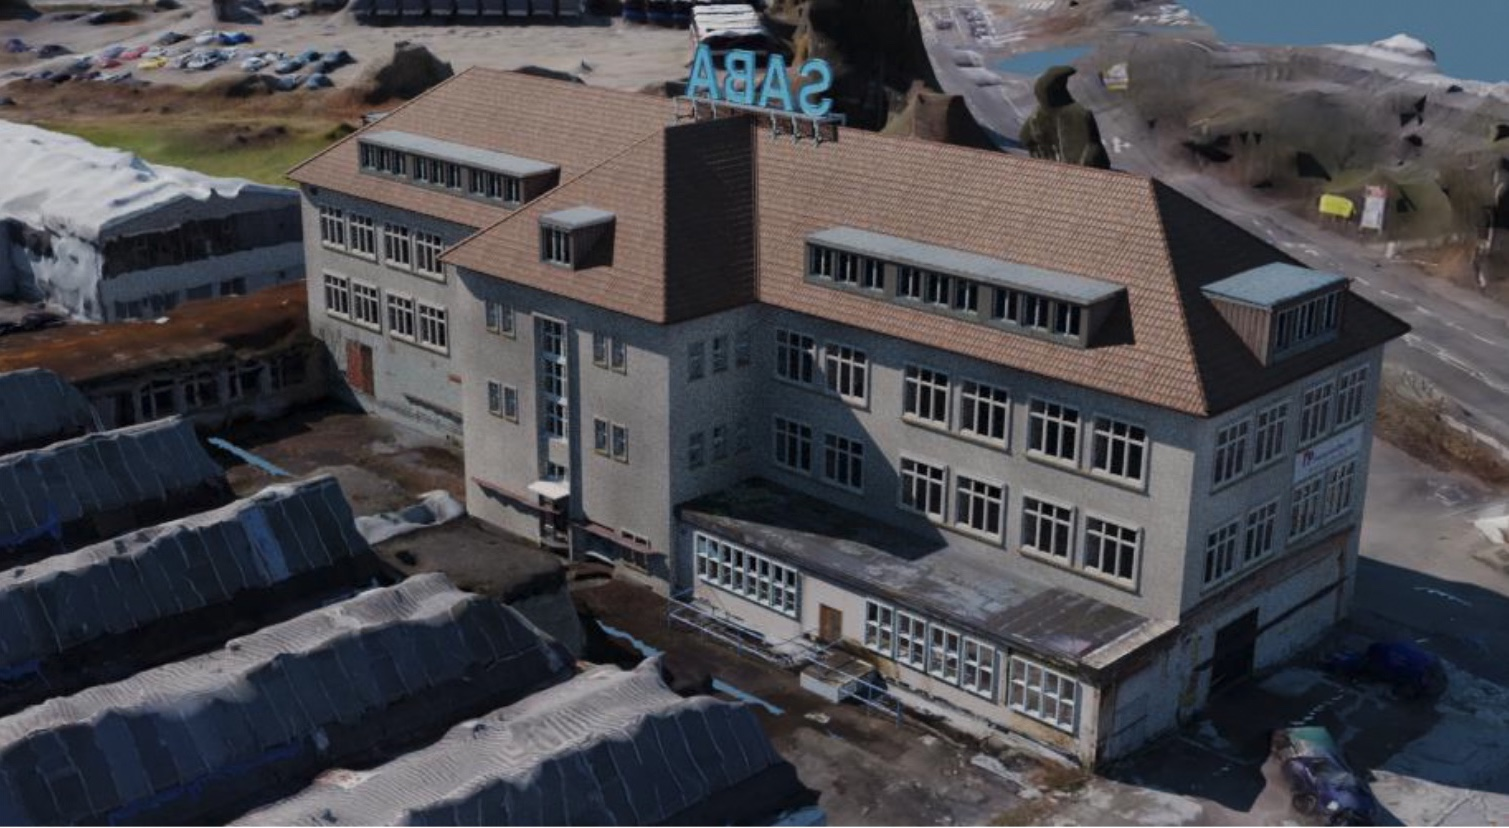
\includegraphics[width=0.6\textwidth]{vorangegangene_Projekte/saba_modell.jpg}
    \caption{Das 3D Modell des SABA Hauptgebäudes in der 3D Karte aus den Drohnen-Aufnahmen.}
    \label{fig:SABA3DModell}
\end{figure}

\subsubsection{Photogrammetrische Aufzeichnungen des Lyautey Geländes}
Im Projekt \textit{NISABA} \cite{nisaba2021} aus dem Sommersemester 2020 und Wintersemester 2020/21 sind 3D Modelle von Gebäuden des ehemaligen Lyautey Kasernengeländes (das heutige "Richthofen") entstanden. Auch in diesem Projekt werden verschiedene Photogrammetrie Programme genutzt. \textit{Meshroom}, \textit{Pix4DMapper} \footnote{https://www.pix4d.com/de/produkt/pix4dmapper-photogrammetrie-software}, \textit{Agisoft Metashape} \footnote{https://www.agisoft.com/} und \textit{WebODM} \footnote{https://www.opendronemap.org/webodm/} weden für dieses Projekt verwendet. Gute Ergebnisse erzielt dabei \textit{Pix4DMapper}, da viele Einstellungen über den Detailgrad getroffen und mehrere Projekte kombiniert werden können. Aus dem generierten Mesh wird auch hier eine Nachmodellierung in \textit{Blender} durchgeführt.

Das Lyautey Gelände umfasst insgesamt sieben Gebäude. Für jedes Gebäude gibt es ein fertiges Modell aus \textit{Pix4DMapper} und ein Modell, bei dem die Polygone reduziert sind. Nur das Manschaftsgebäude gibt es nachmodelliert. Das ist das Gebäude 4 in der Abbildung \ref{fig:lyautey-map}. Alle 3D Modelle können auf der Website des \textit{NISABA}-Projekts \footnote{https://nisaba.villingen-schwenningen.de/uebersicht/} begutachtet werden. 

\begin{figure}[h]
    \centering
    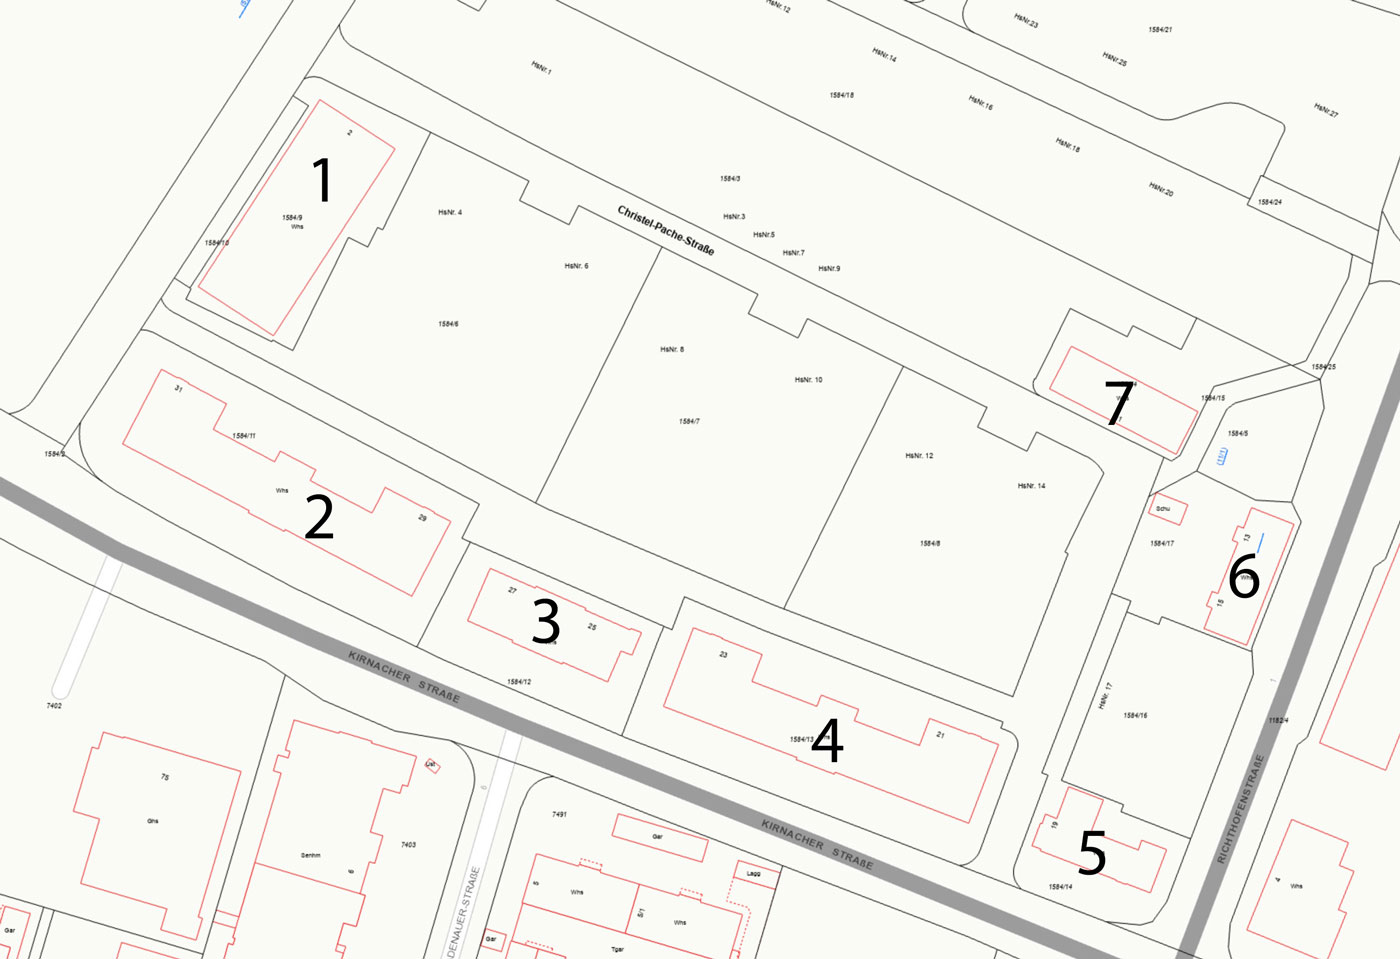
\includegraphics[width=0.8\textwidth]{img/vorangegangene_Projekte/lyautey_map.jpg}
    \caption{Eine Übersicht der Gebäude auf dem Lyautey-Gelände.}
    \label{fig:lyautey-map}
\end{figure}

\subsubsection{Photogrammetrische Aufzeichnungen des Mangin Geländes}
Im Zuge der Veranstaltung Bildverarbeitung und Computergrafik im Sommersemester 2021 im Studiengang Medieninformatik Master sind weitere 3D Modelle entstanden\cite{kusch2021}. Die Gebäude befinden sich auf dem für die Stadt historisch wichtigen Kasernengelände Mangin in Villingen-Schwenningen, das sich direkt östlich vom Lyautey befindet. Dabei handelt es sich um ein verlassenes Kasernengelände mit architektonisch und historisch interessanten Gebäuden. Die Aufnahmen der Gebäude erfolgte in Zusammenarbeit mit dem Vermessungsamt Villingen-Schwenningen. Es wurden Aufnahmen von den Gebäuden 2-8 und 10-12 gefertigt. In der Abbildung x ist eine Übersichtskarte des Geländes mit Nummerierungen der Gebäude zu sehen.  Die Bilder aus der Luft wurden mit einer Drohne vom Vermessungsamt gemacht, während die Aufnahmen am Boden von den Studierenden aufgenommen wurden. Als Photogrammetrie-Software wird hauptsächlich \textit{Pix4DMapper} und \textit{Meshroom} verwendet. 

\begin{figure}[h]
    \centering
    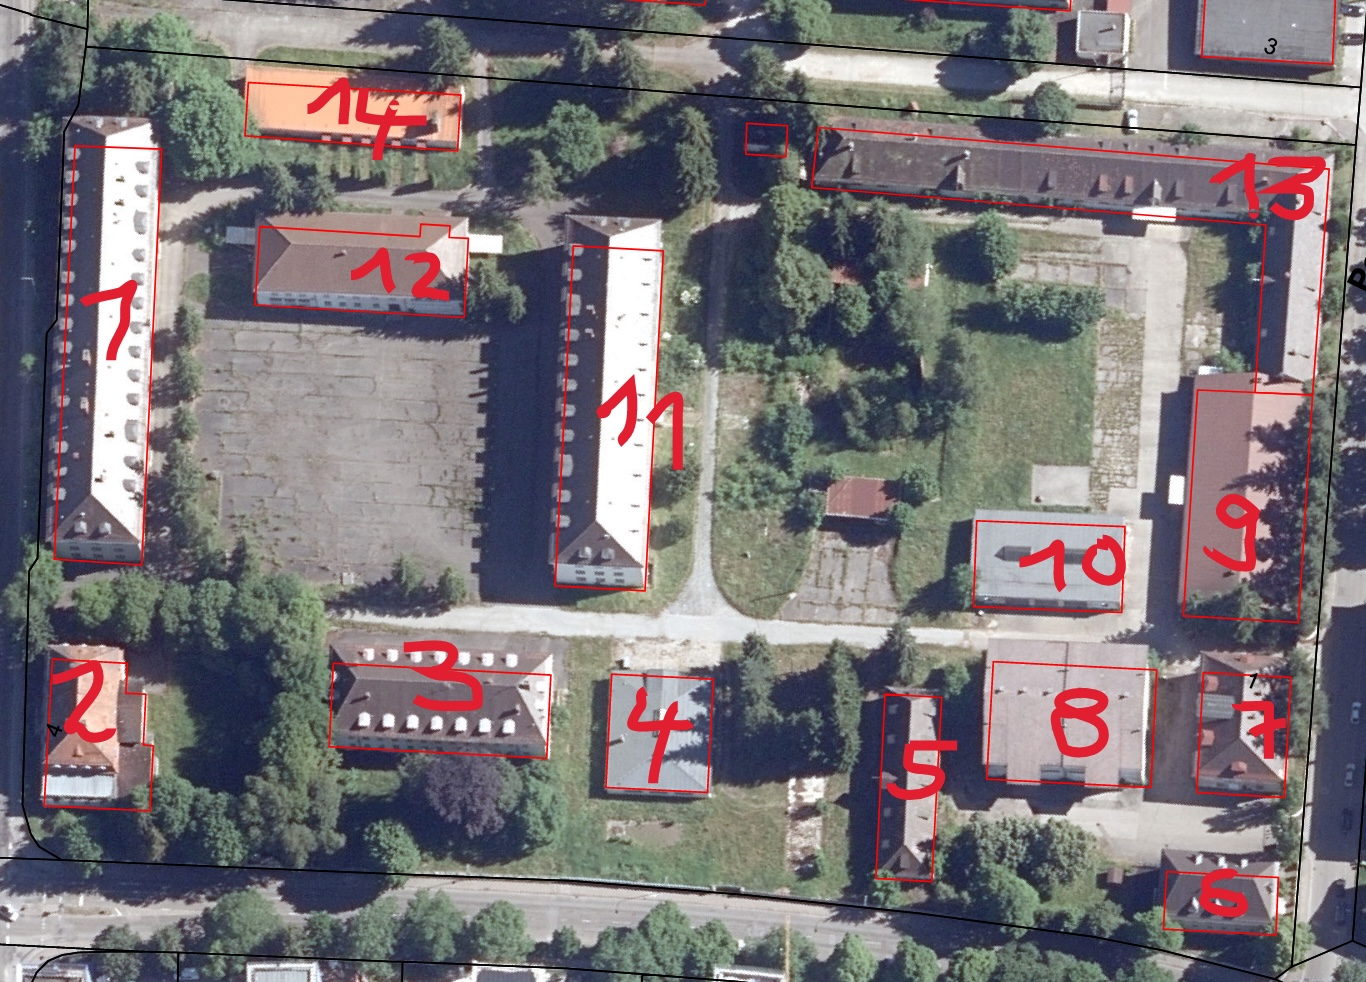
\includegraphics[width=0.8\textwidth]{img/vorangegangene_Projekte/mangin_map.jpg}
    \caption{Eine Übersicht der Gebäude auf dem Mangin-Gelände.}
    \label{fig:mangin-map}
\end{figure}
\subsubsection{Übersicht vorhandener 3D Modelle}
Einige Modelle sind nicht vollständig, haben aufgrund der Vegetation vor Ort Löcher im Mesh oder einen niedrigen Detailgrad. Daher können in dieser Arbeit nicht alle 3D Modelle verwendet werden. Die Tabelle \ref{tab:uebersicht-3Dmodelle} zeigt eine Liste der vorhandenen 3D Modelle. Die Gebäude sind wie in den Übersichtskarten nummeriert. Ein geringer Detailgrad bedeutet, dass das Mesh Löcher hat oder unvollständig ist. Ein mittlerer Detailgrad zeichnet sich durch ein vollständiges Mesh mit geringen Details aus. Gebäude mit einen hohen Detailgrad können für die \Gls{ar} Anwendung genutzt werden. Händisch modellierte Gebäude haben einen sehr hohen Detailgrad.
\begin{table}[h]
    \centering
    \begin{tabular}{|p{0.1\textwidth}|p{0.25\textwidth}|p{0.04\textwidth}|p{0.15\textwidth}|p{0.1\textwidth}|p{0.17\textwidth}|}
    \hline
        Gelände & Bezeichnung                                   & Nr.   & Detailgrad    & Vertices   & Texturenanzahl   \\ \hline 
        SABA    & Karte                                         & -     & gering        & 458.311    & 1                \\ \hline
        SABA    & Hauptgebäude \newline Neumodellierung         & 1     & sehr hoch     & 44.708     & 34               \\ \hline
        SABA    & Heizwerk                                      & 2     & mittel        & 142        & 8                \\ \hline
        Lyautey & Karte                                         & -     & mittel        & 2.049.590  & 1                \\ \hline
        Lyautey & Reithalle                                     & 1     & hoch          & 1.386.531  & 1                \\ \hline
        Lyautey & Mannschaftsgebäude 1                          & 2     & hoch          & 1.255.734  & 1                \\ \hline
        Lyautey & Wirtschaftsgebäude                            & 3     & hoch          & 1.610.983  & 1                \\ \hline
        Lyautey & Mannschaftsgebäude 2                          & 4     & hoch          & 175.352    & 1                \\ \hline
        Lyautey & Mannschaftsgebäude 2 \newline Neumodellierung & 4     & sehr hoch     & 2.046      & 45               \\ \hline
        Lyautey & Stabshaus                                     & 5     & gering        & -          & -                \\ \hline
        Lyautey & Familienhaus                                  & 6     & mittel        & 119.574    & 1                \\ \hline
        Lyautey & Kammergebäude                                 & 7     & hoch          & 269.460    & 1                \\ \hline
        Mangin  & Karte                                         & 1     & mittel        & 502.040    & 1                \\ \hline
        Mangin  & Casino                                        & 2     & mittel        & 681.082    & 1                \\ \hline
        Mangin  & -                                             & 3     & hoch          & 381.633    & 1                \\ \hline
        Mangin  & Pferdestall                                   & 4     & mittel        & 242.984    & 1                \\ \hline
        Mangin  & -                                             & 6     & gering        & 500.463    & 1                \\ \hline
        Mangin  & -                                             & 7     & gering        & 31.490     & 1                \\ \hline
        Mangin  & -                                             & 8     & hoch          & 5.093      & 1                \\ \hline
        Mangin  & -                                             & 10    & hoch          & 500.307    & 1                \\ \hline
        Mangin  & -                                             & 11    & mittel        & 427.753    & 1                \\ \hline
        Mangin  & -                                             & 12    & mittel        & 497.625    & 1                \\ \hline
        Mangin  & -                                             & 17    & gering        & 5.179      & 1                \\ \hline
        Mangin  & -                                             & 23    & gering        & 998        & 1                \\ \hline
        Mangin  & Karte der Gebäude 17-23                       & -     & mittel        & 15.433     & 1                \\ \hline
    \end{tabular}
    \caption{Eine Übersicht der vorhandenen 3D Modelle.}
    \label{tab:uebersicht-3Dmodelle}
\end{table}
